\documentclass[a4paper]{article}

\usepackage[utf8]{inputenc}
\usepackage{amsmath}
\usepackage{amsfonts}
\usepackage{amssymb}
\usepackage{hyperref}
\usepackage{graphicx} % Required for including images
    \graphicspath{{images/}} % Directory in which figures are stored
\usepackage{tabu}
\usepackage{lipsum}
\usepackage{tocloft}
\usepackage{indentfirst}
\usepackage{array}
\usepackage{longtable}
\usepackage{hyperref}
\usepackage[table]{xcolor}

\newtheorem{theorem}{Theorem}[section]
\newtheorem{lemma}[theorem]{Lemma}
\newtheorem{proposition}[theorem]{Proposition}
\newtheorem{corollary}[theorem]{Corollary}
\newtheorem{conjecture}[theorem]{Conjecture}
\newenvironment{proof}[1][Proof]{\begin{trivlist}
		\item[\hskip \labelsep {\bfseries #1}]}{\end{trivlist}}
\newenvironment{definition}[1][Definition]{\begin{trivlist}
		\item[\hskip \labelsep {\bfseries #1}]}{\end{trivlist}}
\newenvironment{example}[1][Example]{\begin{trivlist}
		\item[\hskip \labelsep {\bfseries #1}]}{\end{trivlist}}
\newenvironment{remark}[1][Remark]{\begin{trivlist}
		\item[\hskip \labelsep {\bfseries #1}]}{\end{trivlist}}
\newcommand*{\QED}{\hfill\ensuremath{\blacksquare}}
\renewcommand{\arraystretch}{1.5}
\tabulinesep = 2mm
\setcounter{section}{-1}
\setlength{\arrayrulewidth}{0.5mm}
\setlength{\tabcolsep}{18pt}
\let\tempone\itemize
\let\temptwo\enditemize
\renewenvironment{itemize}{\tempone\addtolength{\itemsep}{-5pt}}{\temptwo}
\pagenumbering{gobble}

\title{
\includegraphics[width=1.1\textwidth]{logo-company}
Automated Compliance Technologies}
\author{White Paper - Version 14}
\date{May 22, 2018}

\begin{document}
\clearpage

\maketitle
\clearpage
\pagenumbering{arabic}
\section*{\centerline{Abstract}}
The exponential growth in electronic commerce and the accelerating evolution of the crypto economy\footnote{\href{https://www.bloomberg.com/news/articles/2018-03-18/growth-of-crypto-assets-may-threaten-financial-system-fsb-says}{https://www.bloomberg.com/../growth-of-crypto-assets-may-threaten..}} increasingly necessitate identity validation\footnote{\url{https://hackernoon.com/kyc-aml-and-cryptocurrencies-4e4cf929c151}} of the parties involved in both centralized and decentralized business transactions. 

Ocular is developing a compliance and onboarding platform that leverages cutting edge technologies such as artificial intelligence(AI) and machine learning to satisfy compliance requirements at the highest possible levels.

Ocular aims to be the de-facto building block for any service that requires identification through KYC for financial applications and onboarding. The process will be fully automated and require little to no interaction from the client. 

Multi purpose and highly customizable, Ocular will typically be used to bridge traditional finance and crypto technologies. It will offer a user-friendly way to verify and validate users in an ecosystem to prevent fraud and expose fraudulent activities. 

Integration of Ocular into any financial or crypto technology platform can be achieved with relatively few changes to clients’ platforms. Ocular also offers stand alone services for authentication and verification. 

The Ocular project consists of three parts. The first, being the cornerstone, is compliance and automated onboarding fueled by our token OKYC. The second is a deep integration with blockchain tech leveraging the capabilities of Ocular with that of distributed ledgers. The third is empowering other cryptocurrency and financial services by offering automated onboarding. Strategic partners implementing Ocular for compliance will then be able to offer fully automated issuing of financial services such as bank accounts, credit cards, exchanges, peer-to-peer payments etc without worrying about complex compliance legal liabilites. 

\pagebreak

\tableofcontents

\pagebreak

\section{Important Notice}
This document and information contained herein may not be sent and or addressed wholly or in part, directly or indirectly, to any person in [the United States or the People’s Republic of China or Saint Kitts \& Nevis], or any other jurisdiction in which it would be impermissible or restricted to offer, distribute, purchase, sell or retain cryptographic tokens.

PLEASE READ ALL PARTS OF THIS NOTICE CAREFULLY. THIS WHITEPAPER IS TO BE READ IN CONJUNCTION WITH THE TOKEN SALE AGREEMENT/TERMS AND CONDITIONS. THOSE DOCUMENTS MAY BE FOUND AT OUR WEBSITE \footnote{\url{https://oculartech.io/token-sale-agreement-terms-and-conditions}}.

All definitions contained in this notice shall bear the same meaning as provided in the whitepaper unless stated otherwise.

The OKYC is not intended to constitute:
\begin{enumerate}
\item securities in any jurisdiction;
\item currency of any kind;
\item stocks, shares, or debentures;
\item units in a collective investment scheme or business trust;
\item equity in an investment fund.
\end{enumerate}

Any regulation or legislation applicable to securities or to any of (1 to 5) above will not be applicable to this Whitepaper and the OKYC Token Offering. This Whitepaper does not constitute a prospectus or offer document, nor is it an offer of securities or an attempted solicitation for investment in securities in any jurisdiction. This Whitepaper and the OKYC Token Offering have not been approved by any regulatory body in any jurisdiction. It should not be assumed that the Whitepaper, or the OKYC Token Offering, complies with any laws, regulation or legislation of any jurisdiction.

The purchase of the OKYC and participation in the OKYC token offering is inherently risky. No warranty, guarantee or undertaking is made by Ocular (Ocular Global LLC) and/or the distributors of the OKYC regarding:

\begin{enumerate}
\item the performance of the OKYC;
\item the performance of the assets underlying the Ocular business or the OKYC token purchase;
\item the accuracy of the information contained in this Whitepaper;
\item the accuracy of any projections, financial or otherwise, contained in this Whitepaper.
\end{enumerate}

The law and regulation of token offerings is in the process of development and review in most jurisdictions. This lack of clarity surrounding the law and regulation further increases the risk associated with the OKYC purchase. As a potential purchaser it is assumed that you have familiarized yourself with the underlying technology and workings of token purchases, blockchain technology, digital wallets and cryptocurrency. It is assumed that you, as a potential purchaser, have the knowledge and understanding of the foregoing and that you have familiarized yourself with the risks associated therewith.

Any agreement between you and Ocular and/or any distributor, in relation to the sale and purchase of the OKYC, will be governed by a separate Token Sale Agreement setting out the terms and conditions of such agreement. In the event of any inconsistencies between the Token Sale Agreement and this Whitepaper, the Token Sale Agreement shall prevail. To the maximum extent permitted by the applicable laws, regulations and rules, Ocular and/or any distributor shall not be liable for any indirect, special, incidental, consequential or other losses of any kind, in tort, contract or otherwise (including but not limited to loss of revenue, income, personal savings or profits, and loss of use or data), arising out of or in connection with any acceptance of or reliance on this Whitepaper or any part thereof by you and any purchase of the OKYC tokens by you.

As a potential purchaser of the OKYC you agree and acknowledge that:

\begin{enumerate}
\item you are recognized as an Accredited/Sophisticated/High Net Worth Individual/Investor in your home jurisdiction; 
\item the purchase of OKYC is inherently risky; 
\item the law and regulation in relation to token offerings, cryptocurrency, digital wallets and blockchain is in the process of being developed and reviewed in most jurisdictions;
\item Ocular and/or any distributor gives no representations, warranties or undertakings regarding the success of the OKYC token offering, the underlying Ocular business, the accuracy of the information and accuracy of the financial/other projections contained in this Whitepaper;
\item to the full extent permitted by the applicable laws, regulations and rules, Ocular and/or any distributor shall not be liable for any indirect, special, incidental, consequential or other losses of any kind, in tort, contract or otherwise (including but not limited to loss of revenue, income, personal savings or profits, and loss of use or data), arising out of or in connection with any acceptance of or reliance on this Whitepaper or any part thereof by you and any purchase of the OKYC tokens by you.
\end{enumerate}

Ocular is committed to providing a safe, compliant and reputable service to our customers. For this reason, Ocular insists on a comprehensive and thorough Know Your Customer (KYC) and anti-money laundering (AML) / combating the finance of terrorism (CFT) compliance implementation. This includes the monitoring of suspicious transactions and obligatory reporting to local regulators and other compliance bodies. Our policies in this regard differ depending on the country of origin of which our clients are located. The specific AML/CFT and KYC policies as per regional jurisdiction are located in the terms and conditions of the Token Sale Agreement. Our compliance framework ensures that regulatory requirements are being adhered to at both a local and global level, instilling a level of trust and ensuring Ocular will continue to operate uninterrupted. Ocular reserves the right to refuse to offer OKYC to persons from or in jurisdictions that do not meet international AML/CFT standards or could be considered as a Politically Exposed Person.
\clearpage
\centerline{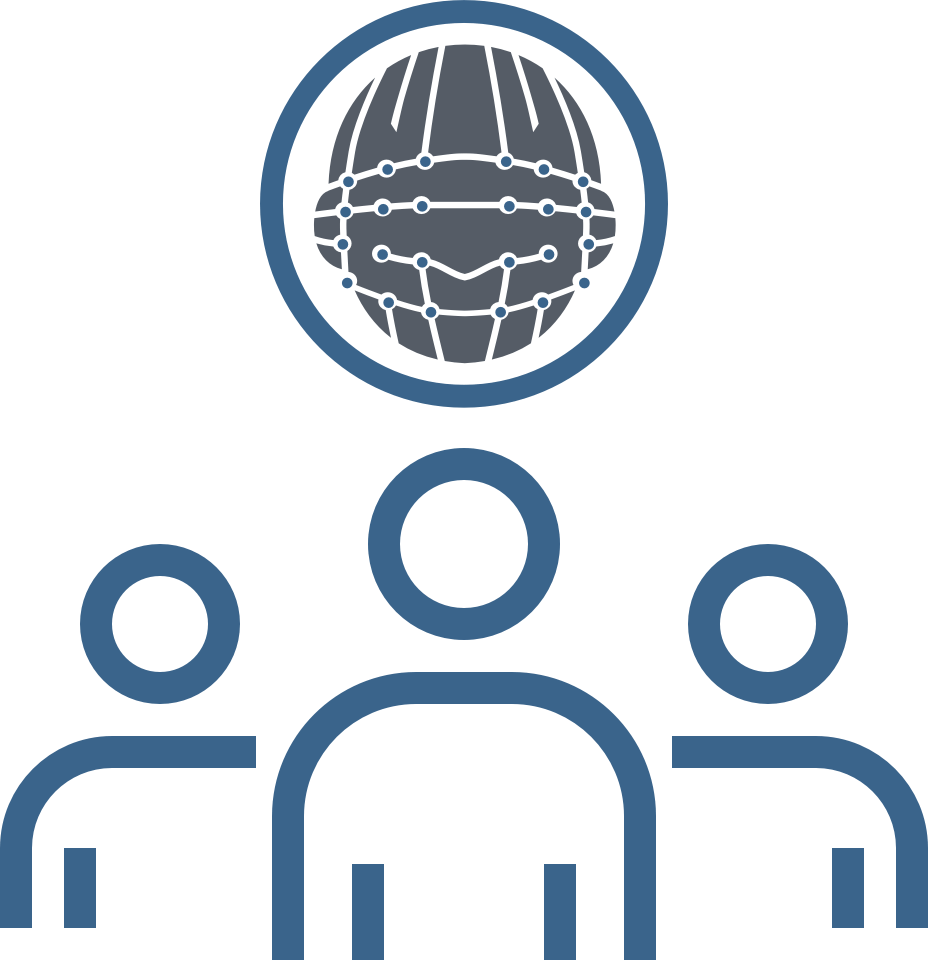
\includegraphics[width=1.0\textwidth]{ocular-kyc-aml}}

\section{Motivation}
Emerging blockchain technologies are ushering in a new economic and social paradigm\footnote{\url{https://www.forbes.com/sites/steveolenski/2018/03/12/what-the-blockchain-revolution-means-for-cmos/}} that will rival the invention of the monetary system. 

The exponential growth in the crypto economy has increased the need for effective compliance services. Fraud, money laundering, online crime and identity theft are on the rise at unprecedented rates\footnote{\url{https://news.bitcoin.com/9-million-day-lost-cryptocurrency-scams/}}. 

Regulators around the world recognize the disruptive potential and are evaluating control mechanisms\footnote{\url{https://www.coindesk.com/eu-regulators-discuss-crypto-regulation-next-week/}} to not only protect the public but also the very governments they represent. Such efforts range from simple guidelines for best practice to outright bans. 

Cryptocurrencies have largely been developed outside of regular centralized channels and compliance measures have not been an integral part of the evolution. In fact, blockchain technology has been fueled by a healthy distrust for authority. Compliance in decentralized systems can be seen by some as undermining the freedom to control one’s own assets and defeating the very principles underpinning the crypto movement. 

Finding a middle ground between these extremes helps the crypto evolution by allowing new disruptive technologies to thrive while following basic rules of compliance. This creates a win-win situation for all constituents and allows crypto to evolve, rather than inducing regulators to shut it down in its infancy. Integrating safety mechanisms such as KYC/AML will allow real, wide scaling across financial services and drive adoption to new heights. 

Exchanges\footnote{\href{https://uk.reuters.com/article/uk-usa-sec-crypto/u-s-regulator-urges-registration-of-cryptocurrency-exchanges-idUKKCN1GO2D0}{https://uk.reuters.com/../u-s-regulator-urges-registration-of-cryptocurrency-exchanges..}} and Token Offerings\footnote{\href{https://cointelegraph.com/news/sec-hints-at-tighter-regulation-for-icos-smart-policies-for-true-cryptocurrencies}{https://cointelegraph.com/news/sec-hints-at-tighter-regulation..}}\footnote{An Token Offering is a fundraising mechanism in which new projects sell their underlying crypto tokens in exchange for bitcoin and ether. ... These are a relatively new phenomenon but have quickly become a dominant topic of discussion within the blockchain community.} – are very likely to be subjected to fierce restrictions as the market is flooded with darker/grey area parties that introduce varying degrees of very real risk and liabilities. 

2017/18 has seen an exponential demand for timely and efficient compliance onboarding measures.  Large exchanges will likely continue to be unable to onboard, Token Offerings will continue to be delayed and services will shut down due to the lack of proper compliance solutions. Often applications are handled manually and with exorbitant fees, often they are not provided at all.  

This opens up a tremendous opportunity, to fill this void, for a startup company with a complete compliance onboarding solution that facilitates the measures needed for the acceleration of this ecosystem. 

Typically, regulators and traditional financial services in the banking sector have not only been hesitant but also directly hostile towards the whole cryptocurrency movement at times. There seems to be a gradual shift, however, in the direction of acceptance under certain conditions. 

There is strong demand for a provider that can not only offer the essential compliance building block of any crypto service but also a bridge to the traditional world of finance, undisputedly based on fiat currency.  

\clearpage
\centerline{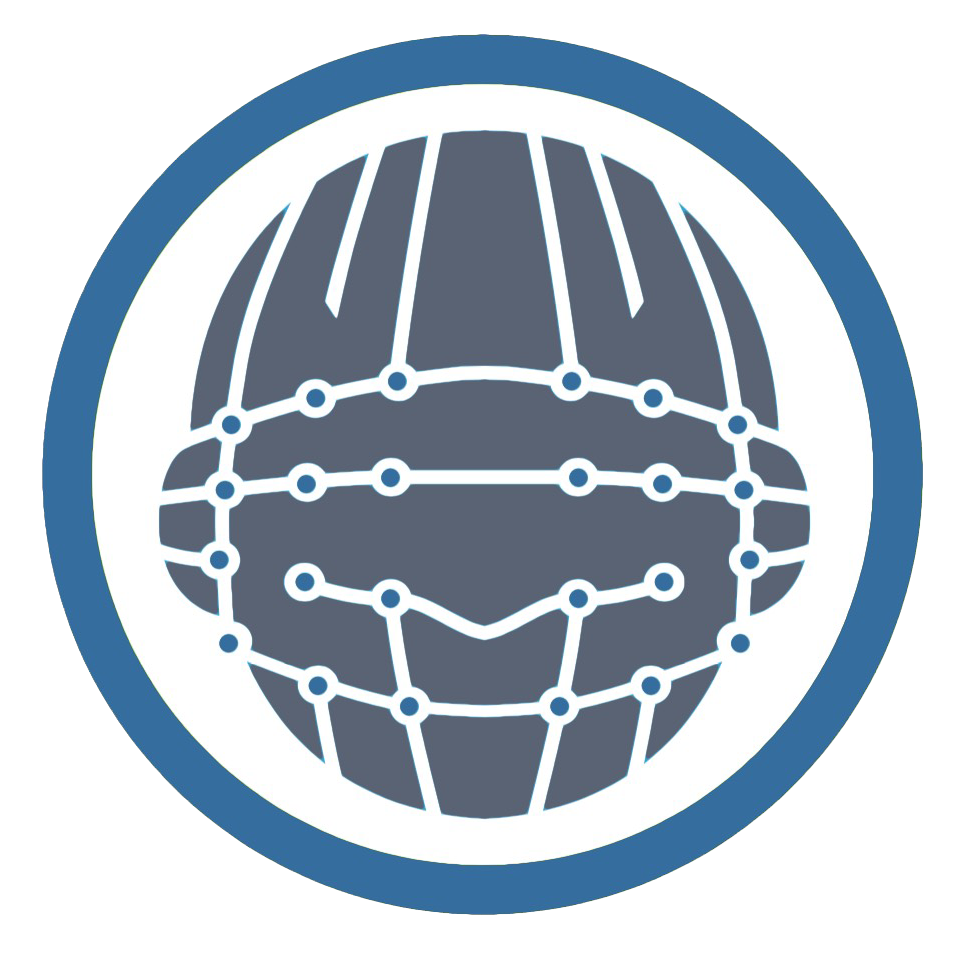
\includegraphics[width=1.0\textwidth]{ocular-head}}
\section{Solution}
Ocular aims to provide a much needed platform that fills the crypto compliance void and accelerates the crypto evolution by providing the following features. 

\begin{enumerate}
\item A first of its kind platform and cryptocurrency for compliance, verification, authorization and identity that facilitates enhanced, efficient customer onboarding for crypto services.
\item Expedited compliance reviews in orders of magnitude by automating a traditionally manual process in a very user-friendly manner.   
\item Fully integrated traditional name and personal data background checks with state-of-the-art identity verification mechanisms such as facial and voice recognition, along with safeguards against ID theft, false registrations, Sybil attacks and other vulnerabilities which compromise and circumvent compliance. Customer data is run through an extensive list of databases in seconds, including OFAC\footnote{The Office of Foreign Assets Control (OFAC) of the US Department of the Treasury administers and enforces economic and trade sanctions based on US foreign policy and national security goals against targeted foreign countries and regimes, terrorists, international narcotics traffickers, those engaged in activities related to the proliferation of weapons of mass destruction, and other threats to the national security, foreign policy or economy of the United States. OFAC acts under Presidential national emergency powers, as well as authority granted by specific legislation, to impose controls on transactions and freeze assets under US jurisdiction. Many of the sanctions are based on United Nations and other international mandates, are multilateral in scope, and involve close cooperation with allied governments.}, Interpol, CIA and FBI, among several others\footnote{The list is quite extensive and only the most relevant are listed here.}. Proprietary technology allows Ocular to quickly capture and validate IDs from over a hundred countries. 
\item API/webhooks integration \footnote{Will be found at \url{https://api.oculartech.io}} and a stand-alone system \footnote{\url{https://kyc.oculartech.io}}. 
\item An unparalleled 3-factor biometric authentication\footnote{Three-factor authentication(3FA) – in addition to the previous two factors, the third factor is “something a user is.” Examples of a third factor are all biometric such as the user's voice, hand configuration, a fingerprint, a retina scan or similar.} and ID program that validates a user with facial and voice recognition.
\item Privacy for transactions between any two parties. Neither buyer nor seller need to know each other’s identity. Counterparty information is validated by Ocular’s system but remains discrete to each user. This allows for privacy between participants in a transaction while still validating the safety (and information) of all parties. 
\end{enumerate}

The Ocular system allows blockchain startups and established blockchain businesses to avoid associations with known criminals or undesirable individuals. The Ocular technology denies criminals access and prevents abuse, while facilitating the services for honest individuals. 

Ocular’s core technology was originally developed for the highly competitive and extremely regulated money exchange industry that has had a long history of being targeted by money launderers.\footnote{The 35 remittance centers along the US/Mexico border between San Ysidro and Tijuana comprise the real-world laboratory for the technology designed to track and subsequently thwart the money laundering practice known as structuring, the act of breaking up financial transactions to circumvent US Federal reporting requirements required for transactions over a specific amount
of money. 33 of the 35 locations employ the Baja XE POS for tracking both cash transactions along with the customers involved in the transactions. This network is what strengthens the BajaXE platform along this border. After 18 months in operation, the US government has determined that the practice of structuring has been reduced at this border by more than 78\%.}

Ocular already has some highly competitive technology for the existing centralized marketplace and applies this together with over a decade of compliance experience to produce a cutting edge platform. This has the unique potential to establish itself as the de facto standard for compliance services for the entire crypto ecosystem, especially Token Offerings and exchanges. Ocular help protect such organizers from being unwittingly used as a vehicle for money laundering and has accurate mechanisms for avoiding jurisdictions that have yet to accept the crypto revolution. 

The Ocular project will be carried out in phases. Below is a basic summary. Please consult our website for an exact roadmap and timeline.

\begin{enumerate}
\item \textbf{Compliance through KYC and fully automated onboarding, and basic 3FA}. Ocular will also develop AML tools for parties in need of deep integration and additional layers of protection. 

\item \textbf{Deep integration with blockchain tech}. We will leverage the capabilities of Ocular with that of distributed ledgers in general. We will form partnerships with other existing projects if it betters our project. At this stage, we will further develop our 3FA system for online identity authentication and verification. 

\item \textbf{Empowering other cryptocurrency and financial services by offering automated compliance.} Strategic partners implementing Ocular for compliance will be able to leverage this technology to fully automated issuing of financial services such as bank accounts, credit cards, exchanges both fiat and crypto, peer-to-peer payments etc with a full anti-money laundering program with processes that will meet or exceed industry standards. 


\end{enumerate}

Ocular's main goal is to create the essential core building blocks that underly most modern financial services such as compliance through KYC/AML, authentication, identity services etc. Ocular empower other projects and help the crypto ecosystem at large. The OKYC token will be necessary to access all the services provided by the Ocular system.

\clearpage

\centerline{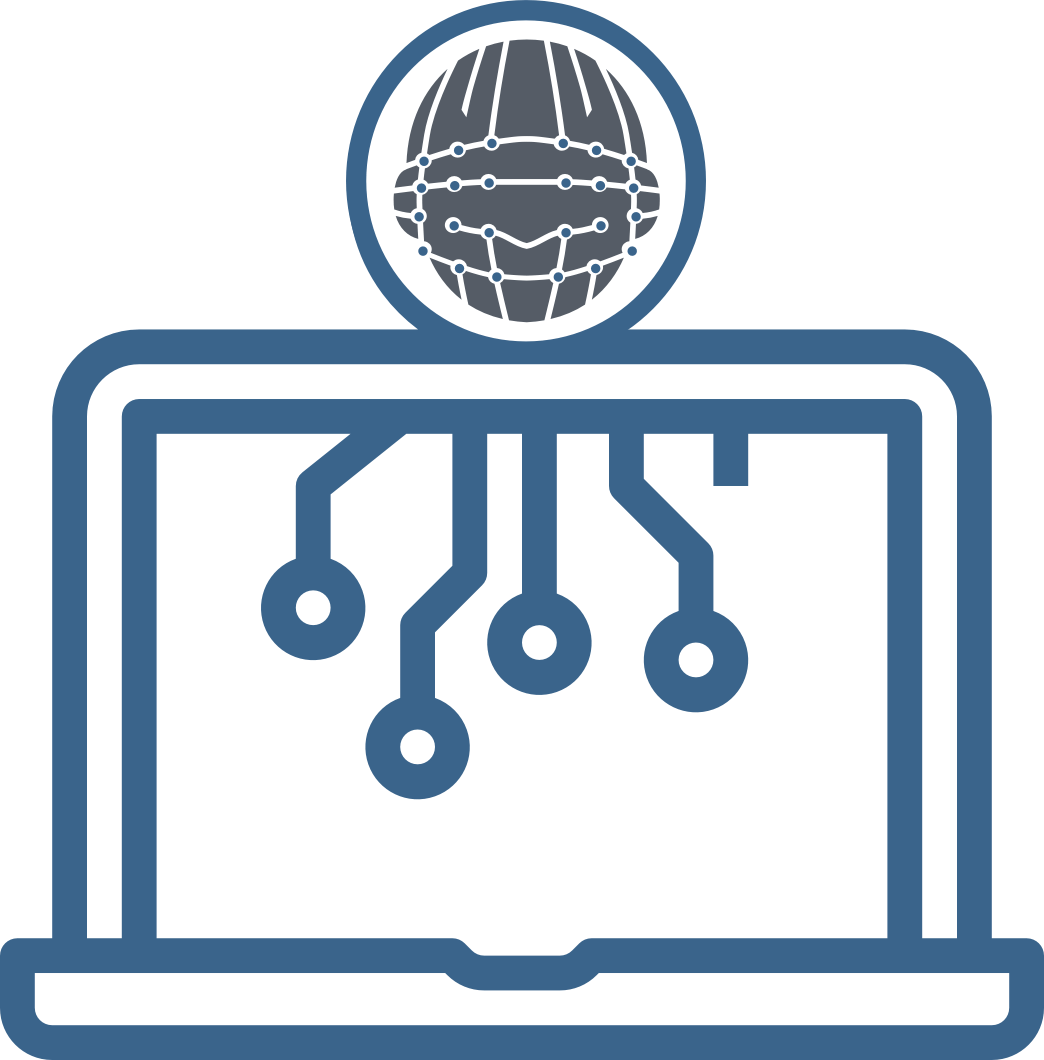
\includegraphics[width=1.0\textwidth]{ocular-crypto}}

\section{Ocular Platform}
\subsection{Modular, Secure Approach}
\subsubsection*{Automatic onboarding for services: token offerings and exchanges}
Ocular will offer a modular approach where various configurations of the platform can easily be integrated into any existing service through \textbf{webhooks}. The onboarding is a fully automated process \footnote{there are some exceptions for banks and accredited investors} where Ocular will take advantage of its compliance tools such as OFAC as well as AI and machine learning for facial/voice recognition. 

By collecting a wide range of data points, we calculate a risk matrix that forms the basis for the approval process. High risk score or other red flags will alert either our compliance officers or the administrators of the service integrating Ocular to take a closer look depending on what sort of integration the service utilizes.

\subsubsection*{3-Factor Authentication that integrates with ID services}
Rather than reinventing yet another ID platform Ocular wants to build tools that can be the very engines across all platforms. Our 3FA solution is powered by the Ocular compliance engine and facial/voice recognition is used for authentication/verification. This will offer a secure solution which is essential when handling one's crypto assets and interfacing with services such as exchanges. Most services can integrate this technology with little to no changes to their existing platform. 


\subsubsection*{Settlement layer for all our compliance services through our token OKYC}
All settlements on the platform are fueled by the OKYC token. 

\subsubsection*{Decentralized compliance verification}

While adhering to strict legal data sharing regulations, the platform will allow for validators to verify parts of the data submitted, and the token OKYC will be used to incentivize external verifiers to provide such services.

\subsubsection*{Special applications}
The platform will handle accredited investors and other special considerations for markets such as the US. Manual tasks that cannot be automated will be handled by external validators or our compliance officers. 

\subsubsection*{AML tools}
Anti-money-laundering system with real-time alerts, velocity checks, tracking and reporting. Read more about AML in a section later on.

\subsubsection*{Lobby cameras}
Facial recognition security system already being widely used in locations around the world.

\subsubsection*{Supported platforms}

Ocular will support computers with a camera and most iPhone/Android compatible handheld devices through native applications. Focus is on a simple yet intuitive interface that allows for a smooth and responsive user experience.

\subsubsection*{Sybil attack protection}

Through advanced algorithms powered by artificial intelligence and machine learning, Ocular will offer various screening features that are fully configurable. For example, the system can be randomly asked for the selfie to be taken with one eye closed, one finger raised etc. to ensure that the data captured is live and to protect against Sybil\footnote{A Sybil attack is an attack where a single adversary is controlling multiple nodes on a network. It is unknown to the network that the nodes are controlled by the same adversarial entity. For example, an adversary can spawn up multiple computers, virtual machines, and IP addresses. They can create multiple accounts with different usernames and e-mail addresses and pretend that they all exist in different countries.

Avoiding Sybil attacks is a difficult problem. In centralized systems they are typically avoided through heuristics that do not provide cryptographic assurance of Sybil resilience. For example, a centralized entity may try to avoid Sybil attacks by requiring that an individual IP cannot create more than a specific number of user accounts in a given time interval.

Sybil attacks are avoided in Bitcoin by requiring block generation ability to be proportional to computational power available through the proof-of-work mechanism. That way, an adversary is limited in how many blocks they can produce by their total computational power. This provides strong cryptographic guarantees of Sybil resilience.} attacks and other hacks designed to game registration processes. 

\subsubsection*{Automatic onboarding for traditional financial services such as Bank Accounts and Credit Cards}
Partners implementing Ocular technology can leverage this to automate issuing of traditional Bank Accounts or even Credit Cards as our systems and compliance officers follow international rules for compliance by the book and more.. Ocular also applies tools such as AML and additional database checks as additional security.

\subsection{Basic user action flow and interaction with Ocular}
\centerline{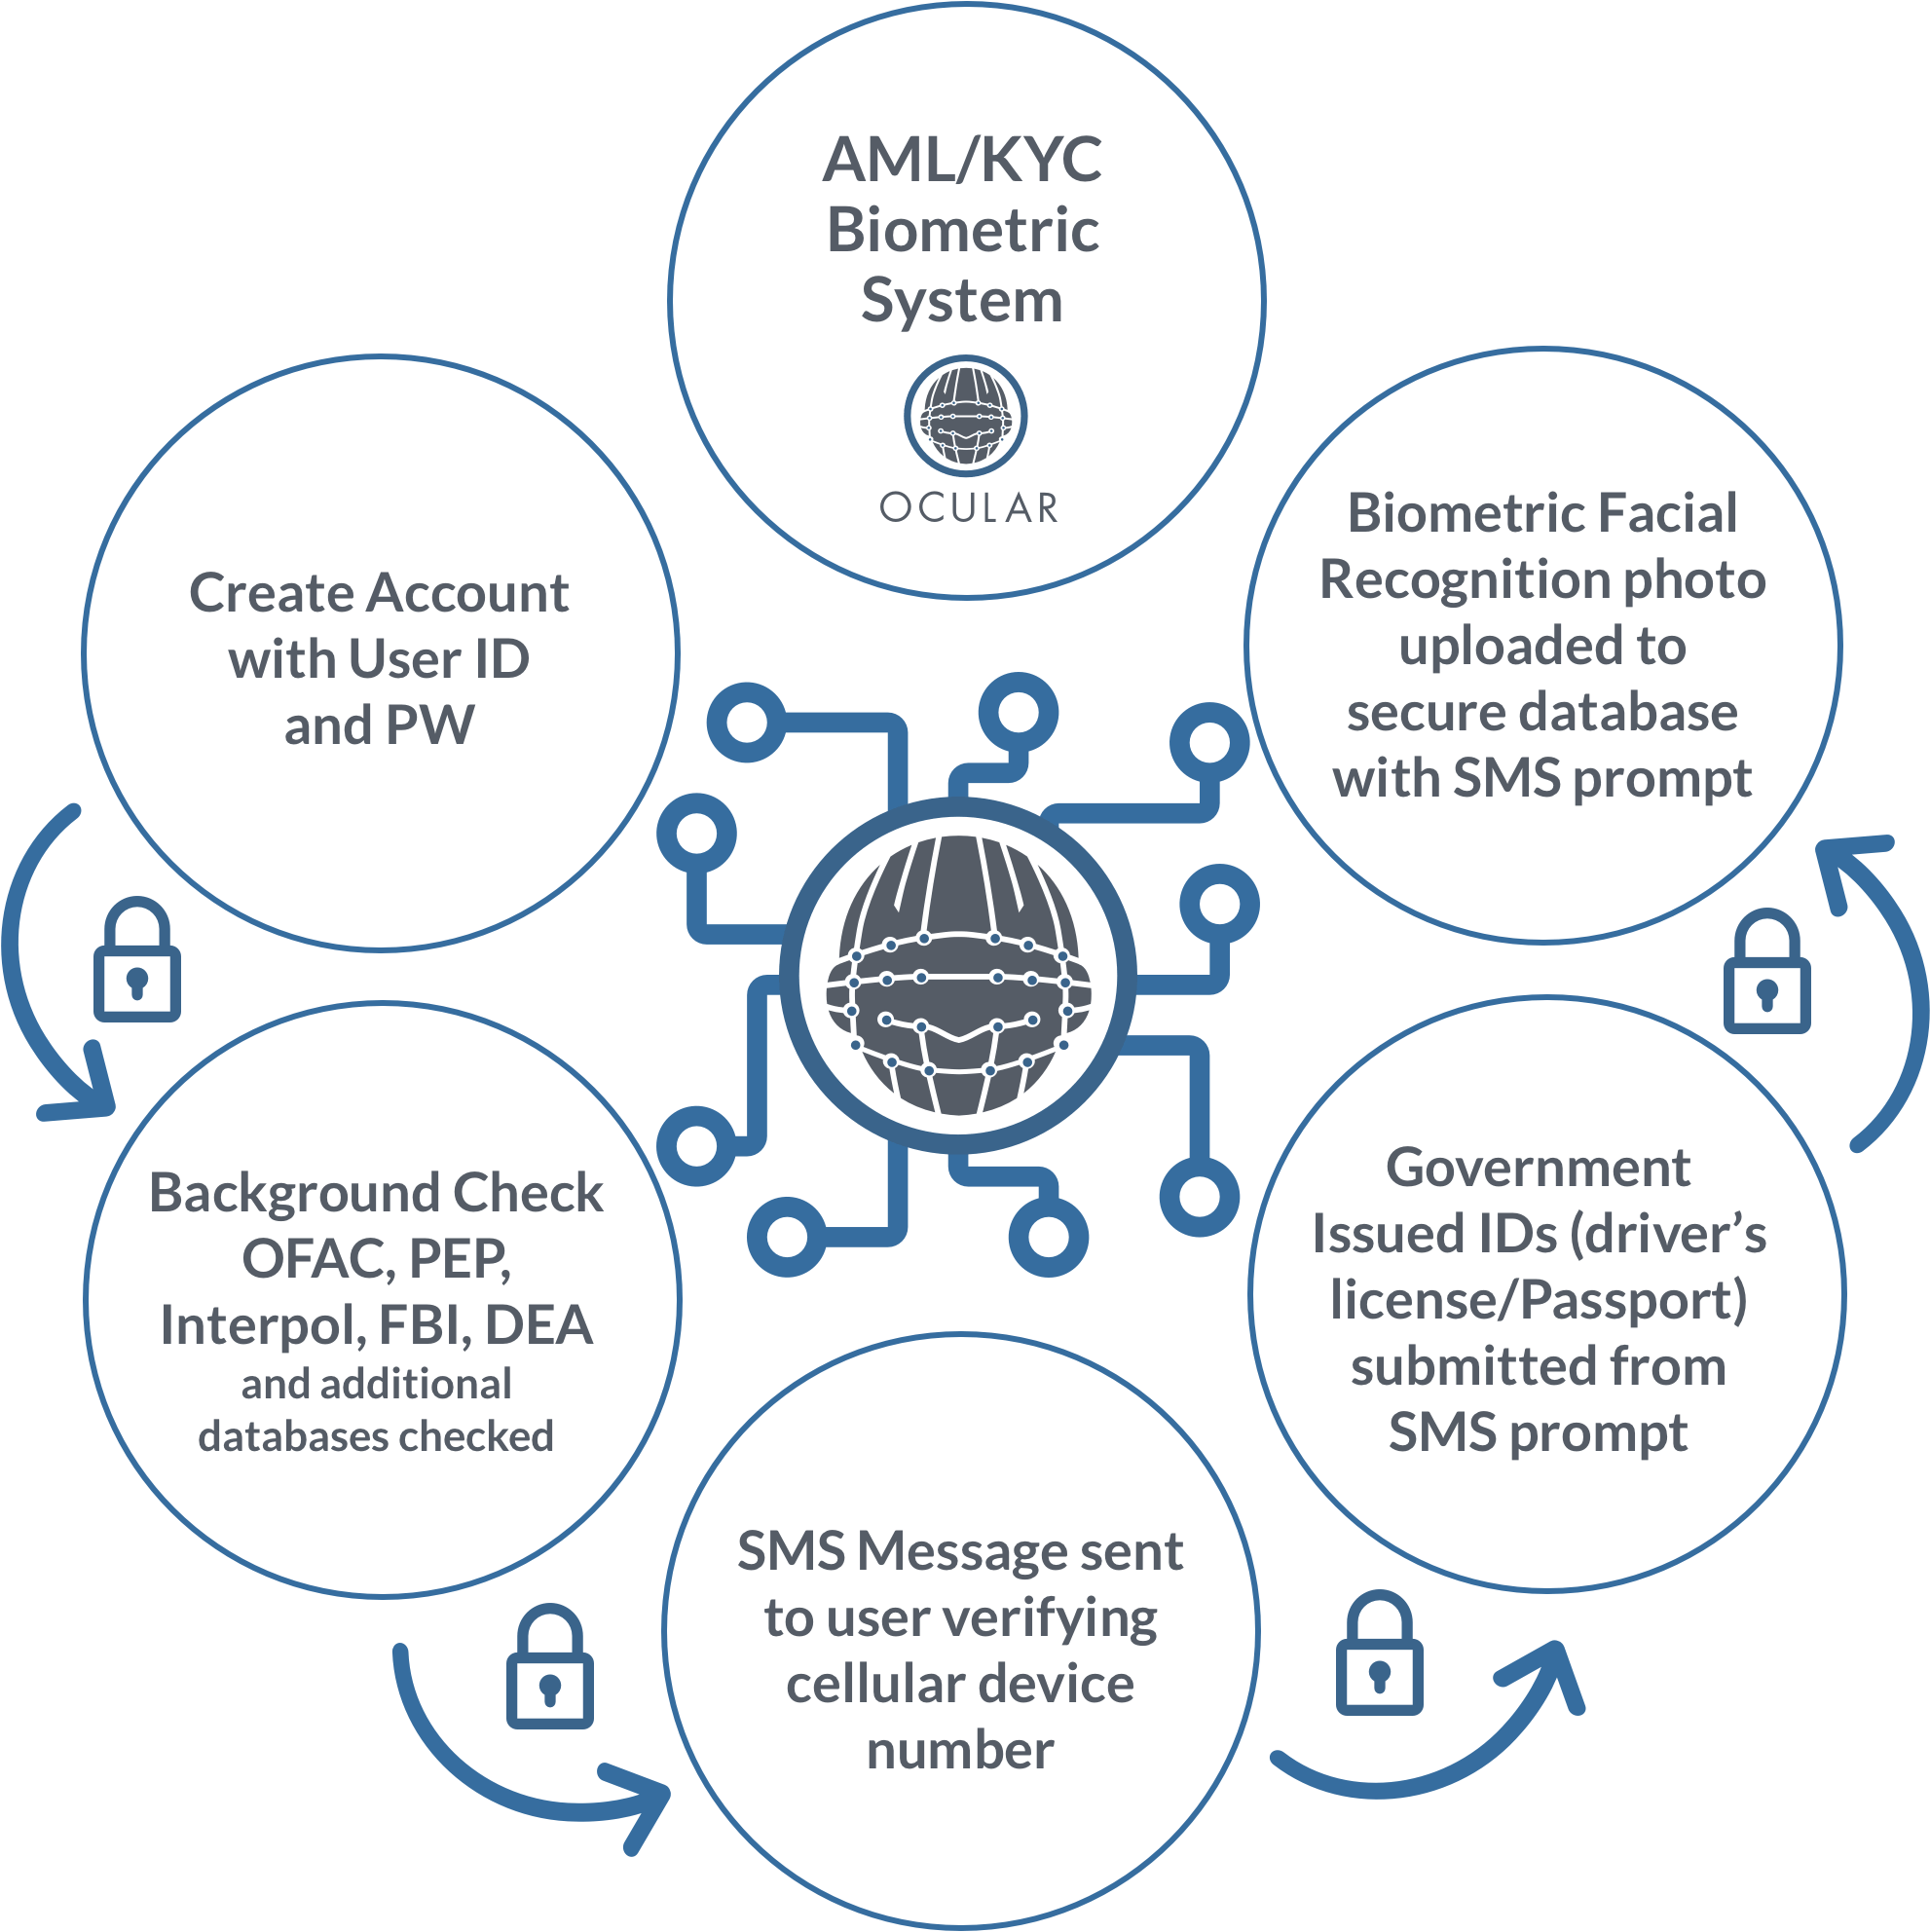
\includegraphics[width=1.1\textwidth]{biometric2}}
\begin{enumerate}
\item The user creates an account with user identification.
\item The platform enables an automatic and instant check on OFAC (Office of Foreign Assets Control), Interpol, PEP (Politically Exposed Persons) and other worldwide databases and confirms an applicant’s eligibility. The Ocular system can search records within five seconds or less. If the applicant is wanted or banned from doing business, the system will immediately stop the registration process.
\item Users receive an SMS message to verify their cellular number and validate their registered device number.
\item Users upload government issued identification from the SMS prompt. The identification verification involves scanning and authentication of passports from every country, and driver's licenses and national IDs for over 182 countries. This filters out usage of any false identification documents.
\item Ocular uses proprietary facial and voice recognition systems that compare photographs taken at registration with those taken for identification. The system periodically requires users to provide new selfies to confirm the identity of the users. Further, voice recognition stops an individual from entering strawman accounts as it ties the face with the voice to limit registrations to one person per voice.
\end{enumerate}
\subsection{Compliance Processes Overview}
\subsubsection*{Simple Registration}
Ocular uses OCR (optical character recognition) from a picture of an ID. This will leave only a few fields to manually key-in. The entire process including ID verification takes less than 60 seconds.

\subsubsection*{OFAC and Background Check}
The Ocular automated interface with worldwide databases provides clients with confidence that they have completed their required due diligence while satisfying the applicant with a smooth experience. 

\subsubsection*{ID Capture \& Authentication}
Our ID capture and authentication feature can save hours if not days in properly reviewing and vetting prospective applicants. 

\subsubsection*{Facial \& Voice Recognition}
Ocular takes facial recognition to a new level by requesting “random selfie images” and “voice prints.” It compares the files to ones that exist to confirm identities. It also adds elements of these submissions to its file and builds a more accurate file every time an additional image or audio file is added. This helps protect a customer from account fraud.

\subsubsection*{Compare Images}
The Ocular system instantly verifies any uploaded selfie with an applicant’s identification to protect against identity theft.

\subsubsection*{Voice Capture}
Voice capturing allows for verification of new registrants. The Ocular facial and voice database are queried for each new registration so that anyone registering for a second account with a different ID will be stopped. This is particularly valuable for stopping ID farm applications.

\subsubsection*{ID Authentication}
The Ocular app confirms the authenticity of an ID in less than 10 seconds.

\subsubsection*{Store and Use}
Ocular allows clients to offer their customers the option to access their own KYC file for use in registering with other businesses (such as banks) that require customer due diligence. Once a client has a KYC in the system, it can be used with any other Ocular client. This allows for a Single Entry Multi-Use Compliance Profile.

\subsubsection*{KYC - Know Your Customer}
Know your customer\footnote{\url{https://en.wikipedia.org/wiki/Know\_your\_customer}} is the process of a business identifying and verifying the identity of its clients. The term is also used to refer to the bank and anti-money laundering regulations which governs these activities.

\begin{itemize}
\item Find a Person
\item Instant ID Consumer Verification
\item Instant ID Consumer with Red Flags
\item Instant ID Consumer Verification with Fraud Point Score
\item Instant ID Consumer Verification with Red Flags and Fraud Point Score
\item Relationship Finder
\item Lexis/Nexis Identity Report
\item Fraud Point Score with Red Flags Rule Report
\item SSA Verify
\item Lexis/Nexis Phone Finder
\item Phone Lookup
\item OFAC \& Other Watch Lists
\item Statewide Public Records Person Search
\item Driver Licenses
\item Marriage \& Divorce Records
\item People At Work
\item Business Executive \& Political Biographies
\item Professional Licenses
\item Voter Registrations
\item Email Address/Social Network Report
\item Other Customized Search Options Available 
\end{itemize}

\subsubsection*{Custom integration with external databases}
\begin{itemize}
\item Black Lists
\item White Lists
\item Preferred Customer List
\item Frequent Shoppers
\item Transaction Histories
\item Geographic Location Histories
\item Internal Data Mining
\item User Defined Lists 
\end{itemize}

\clearpage


\centerline{
\includegraphics[width=1.0\textwidth]{ocular-creditcard}}

\section{Market Entry}
The Ocular team’s client acquisition strategies have included establishing relationships with networks, experts, and current market suppliers that can best leverage our services and technology. 

Ocular’s initial focus will be on offering much needed compliance multi purpose tools to the cryptocurrency ecosystem including but not limited to token sales and exchanges.

There are many other areas that need various degrees of compliance services such as security companies, locksmiths, Point of Sales and payment processors as well as governments, schools and universities. Our strategic advisors are already targeting such partners with substantial user bases and plan on offering various customizable versions of Ocular tailored to their needs.  
\section{Ongoing R\&D}
Ocular will be the essential building block of other decentralized apps that needs compliance. Rather than building a vertical application with limited expandability, Ocular is constantly researching and developing its ecosystem. Through our expertise combined  with R\&D, Ocular delivers the missing, critical piece that will allow crypto projects to scale and reach wide adoption while also adhering to compliance.
\clearpage

\centerline{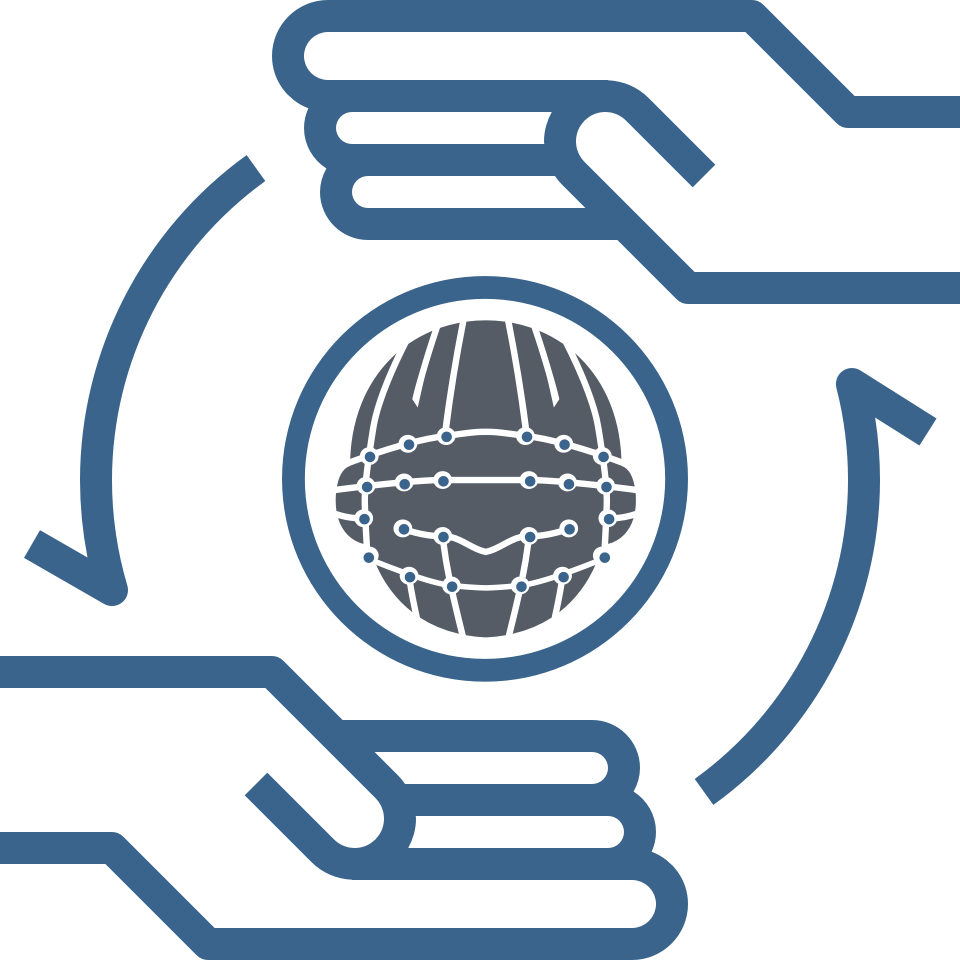
\includegraphics[width=1.0\textwidth]{ocular-exchange}}
\section{Partnerships}
\subsection{Ole Group}
The word “Ole” was originally an acronym for Oil Light Energy. It has evolved to something much more with a history of innovating products and services for its own needs and rolling them out as separate business units.
 
Among the first products to be developed by Ole was “Trade Enabler”, a system that allowed the company to more efficiently process transactions related to its energy assets.

As Ole grew, it developed an accounting system that allowed for international payment capabilities. The system managed vendors, employees and customers and went on to become Ole Pay which is now a licensed money transmitter\footnote{MSB Registration Number: 31000104088710}. 

To address new regulations Ole began developing a compliance program to manage its own operations. This resulted in a biometric based Compliance and Anti-Money Laundering system that is being rolled out worldwide as Ocular.

\subsection{Baja/XE}

Co-developer of Ocular KYC/AML/Facial recognition technology.   


\subsection{Timeline}
Future roadmap found on our webpage \url{https://www.oculartech.io}.
\begin{itemize}
\item Oct 2003: Baja XE goes live – launches a Point of Sale system for managing currency exchange centers integrating both hardware and software, streamlining the capture operations, reducing errors, and preventing money laundering and financing terrorism while following the general provisions referred to in Article 95 of the General Law of Organizations and auxiliary Credit Activities (LGOAAC) applicable to the exchange centers that Article 81-A of the same law concerns.\newline
\\
Milestones completed:
\begin{itemize}
  \item KYC Database searches
  \item Secure storage of transactions
  \item System tracking of individuals
\end{itemize}
\item May 2004: Added capture of Photo (selfie) and Photo ID at the Point of Sale (teller)
\item March 2005: Added Biometric fingerprint scan
\item May 2005: Added additional verification for individuals on restricted lists
\item Nov 2005: Added system alerts; added suspicious transaction activity alerts (AML/Anti Stacking Features)
\item Feb 2007: Remote authorizations added for management
\item January 2008: Added Real time on-line web and mobile device reports
\item March 2009: Certified Bank and money transfer compliance in USA
\item June 2010: Certified Mexico SAT compliance achieved
\item July 2013: CNDD Mexico compliance standard achieved
\item Nov 2015: teamed with Ole Group and GreenBox Compliance to develop tools for the financial services industry. Cash logistics: Provided secure Cash Stations (smart safes), cash reconciliation, cash transportation, deposit, transfer or conversion, and return of Pesos to client to replenish inventory. Cash movement across border approved by both Mexican and US Border authorities.
\item First Face Recognition testing comparing images on file with ID and individual selfie captures. Developed proprietary storage method for images.
\item Jan 2017: Face recognition application tracked with suspicious transactions in money services systems
\item June 2017: Added lobby camera to the system for security alerts. Created DVR conversion for security cameras to add to still image capture file.
\item October 2017: Partnered with Ole, GreenBox and Cryptocurrency Specialists to launch Ocular. Began converting point of sale system features to an e-commerce platform.
\item Nov 2017: Created first Three Factor Authentication process to confirm user identity with selfie.
\item Jan 2018: Begin BOI process in Bangkok, Thailand to set up Ocular Head Quarters
\item Feb 2018: Thailand Office staffing and new support hires launched. Opened office in Bangkok and began hiring process for customer service positions for KYC verifications – minimum of 4 customer support staff needed and ultimately to be expanded to at least 10 staff before June 2018.
\item Began discussions to evaluate Ocular technology for Thailand Immigration.
 \end{itemize}
Future roadmap for the various engines that drive Ocular will be listed on our webpage \url{https://www.oculartech.io} as they will be constantly evolving.
\newpage
\centerline{
\includegraphics[width=1.0\textwidth]{ocular-realestate}}

\section{Token Utility}
The following are use cases for the Ocular OKYC Token: 
\begin{itemize}
  \item Enterprises wishing to validate the authenticity of the credentials of a potential business partner or employee.
  \item Enterprises wishing to purchase tokens for future use cases.
  \item Buyers and potentially end users who will take advantage of the token integration into the ecosystem.
  \item External validators who earn tokens during the process of validating the identity of an individual will use such tokens to exchange for goods and services.
  \item Strategic partners that integrate Ocular supports OKYC as a settlement layer. 
\end{itemize}

%\texttt{This section will be further clarified in next version.}

\centerline{
\includegraphics[width=1.0\textwidth]{ocular-ewallet}}

\section{More about AML}
The cornerstone of a strong AML Compliance program is the adoption and implementation of comprehensive CDD (Customer Due Diligence) policies, procedures, and processes for all customers, particularly those that present a higher risk for money laundering and terrorist financing. The objective of CDD should be to enable the MSB\footnote{A money services business (MSB) is a legal term used by financial regulators to describe businesses that transmit or convert money. The definition was created to encompass more than just banks which normally provide these services to include non-bank financial institutions.} to predict with relative certainty the types of transactions in which a customer is likely to engage. These processes assist the MSB in determining when transactions are potentially suspicious. The concept of CDD begins with verifying the customer’s identity and assessing the risks associated with that customer. Processes should also include enhanced CDD for higher-risk customers and ongoing due diligence of the customer base. Effective CDD policies, procedures, and processes provide the critical framework that enables an MSB to comply with regulatory requirements and to report suspicious activity.

Effective CDD policies, procedures, and processes are critical to an MSB because they can aid in: 
\begin{itemize}
  \item Detecting and reporting unusual or suspicious transactions that potentially expose the bank to financial loss, increased expenses, or reputational risk.
  \item Avoiding criminal exposure from persons who use or attempt to use the MSB’s products and services for illicit purposes.
\end{itemize}

An MSB’s AML guidelines should ensure that the company possesses sufficient customer information to implement an effective suspicious activity monitoring system, paying particular attention to high-risk customers. Under this approach, the MSB should obtain information at account opening sufficient to develop an understanding of normal and expected activity for the customer’s occupation or business operations. If there is indication of a potential change in the customer's risk profile (large, abnormal transactions, change in employment or business operations), the customer’s risk rating should be reassessed at that time. CDD processes should include periodic risk-based monitoring of the customer relationship to determine whether there are substantive changes to the original CDD information (e.g., change in employment or business operations). 

Once policies and procedures are in place to identify, research and report suspicious activities, ongoing monitoring can spot patterns of concern. 
\begin{quotation}For example:
\begin{itemize}
  \item An accountholder who anticipated \$10,000 in weekly cash deposits when they opened the account, has been routinely taking in \$100,000 a week.
  \item A personal account has business-type transactions occurring within it.
  \item A business that is making large routine payments to an unrelated individual or business.
\end{itemize}
\end{quotation}

Ongoing scrutiny is particularly important in the case of customers that pose enough of a money-laundering or terrorist-financing risk to warrant enhanced due diligence. The MSB must clearly understand the anticipated transactions of such clients and use this information in its suspicious-activity monitoring of these customers.

Ocular's AML technology has a track record of use with major financial institutions for several years already and is being redesigned to integrate the security and data privacy afforded by cryptocurrencies and the blockchain. Application of these procedures enhances the safety of our platform and clearly sets us apart.
\newpage

%%%%%%%%%%%%%%%%%%%%%%%%%%%%%%%%%%%%%%%%%%%%%%%%%%%%%%%%%%%%%%%%%%%%%%%%%%%%%%%%%%%%%%%%%%%%%%%%%%

\centerline{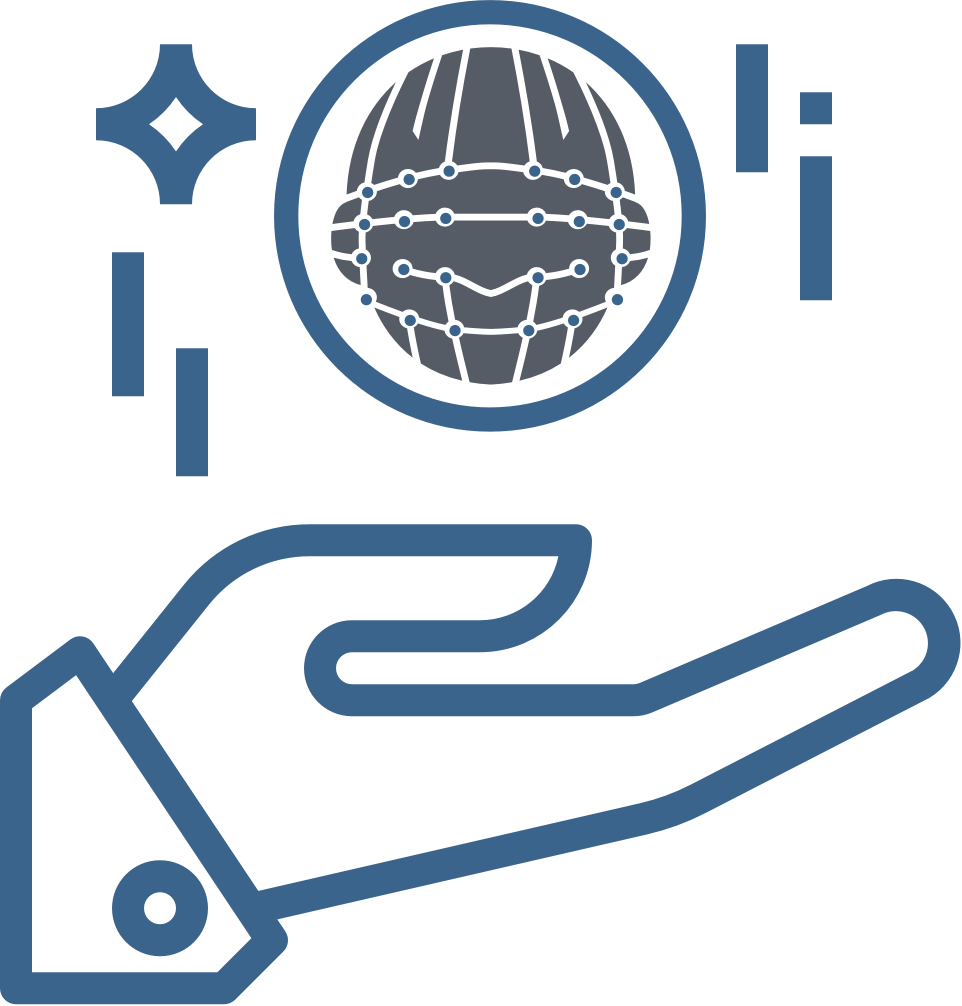
\includegraphics[width=1.0\textwidth]{ocular-pos}}
\section{Token Model}

Ocular proposes a paradigm shift in KYC/AML procedures. Typically, if Organization A requires the data of User B, then User B has to deal with the following security hazards:
\begin{itemize}
\item If online, sending sensitive personal data across unprotected communication channels;
\item Trusting Organization A and the people in charge of handling data at A to not tamper with the data or leak the data;
\item Trusting the security measures undertaken by A to be of sufficient cryptographic hardness; 
\item Finally and perhaps most importantly, the fact that A might not be the sole keeper of the sensitive data, allowing more points of failure potentially. 
\end{itemize}

As a result of the above problems with centralized systems, we have seen countless hacks of data such as medical records and token offering user data. Indeed, it seems likely that hacks will only grow exponentially in the future because of multiple sources of failure with large organizations, both public and private, storing user data. Ocular's ideology is aligned with the future of data privacy, protection and incentivizing honest users and validators of the system.

In the identity layer of the Ocular system, there will be three main participants:
\begin{itemize}
\item Validators
\item Users
\item Services and Service Providers
\end{itemize}
Each participant has specific goals and functions, although the three parties are not mutually independent. 
\subsection{Validators}
The validators are trusted parties that provide verification of user data. Ocular itself is the first validator since the user must provide a variety of details and information to onboard, as described in the previous sections. Validators have the function of forming a cryptographically secure ``attestation'' that is then recorded on the blockchain, in this case the Ethereum blockchain. 

\subsubsection*{Approval Process}
The approval process involves multiple mathematical processes, including mathematical hash functions. Properties of hash functions:

\begin{itemize}
\item Efficiently map data of arbitrary size to a bit string of a fixed size
\item Ideally one-way
\item Collision resistant - i.e. it should not be computationally or mathematically easy to discover $m_1$ and $m_2$ such that $h(m_1)=h(m_2)$. Otherwise, an attacker with a different piece of identification information would be able to act as an impostor for a generic, honest user.
\end{itemize} Hence, given the raw information corresponding to the user data purveyed by the users joining the Ocular system for the first time, say: $$\{u_i\mid\text{each }u_j\text{ corresponds to specific user data }\forall i=1,...,n\}$$ the digests of these data $h(u_i)$ created by provably secure hash functions would prove crucial for demonstrating validators' approval on the blockchain.
The idea is for the users to be in complete control of how much data they send to external validators when information is requested. This can be accomplished in several ways, one of which is to utilize Merkle trees to organize data. In that case, each node in the tree would correspond to a specific subset of user data such that all nodes would eventually be organized into a Merkle root, allowing case-by-case Merkle proofs in the future. In case a certain subset of user data does not occupy a sufficiently large sample space, we can organize that subset with other subsets of user data in the same node, or introduce nonces in order to increase randomness for security purposes and minimize the vulnerability of hashes. In utilizing such a structure overall, the system can provide users with more flexibility and control over their data while allowing tracking of data in a more organized manner.

The other key component to the approval process involves a mathematical digital signature scheme $\sigma(MSG)$ that would demonstrate the authenticity of what is provided by the blockchain. For instance:

\begin{align*}
\sigma &= F(k_{priv}, h(MSG))\\
Verification &= F'(k_{pub}, \sigma)
\end{align*}\\
\begin{align*}
If&: Verification=h(MSG)\\
Then&: \text{the validity of $\sigma$ is proven}\\
If&: Verification\neq h(MSG)\\
Then&: \text{the validity of $\sigma$ is disproven}
\end{align*}

This type of cryptographic scheme is vital in two ways. First, a user in the Ocular system can provide digital signatures to attest to a hash or data on the blockchain. Second, a separate entity can attest to the same data if necessary and provide extra support and authentication on the blockchain. One can prove their private key through cryptographic means in a secure manner without any risk of revealing the key as a result.

At the same time, note that it is always possible to reproduce the hash if and only if using the original raw data. As a result, a user is able to reproduce the hash, if absolutely necessary, to demonstrate to another participant in the network as long as the original data are accessible. This is due to the nature of functions used in the process.

\subsubsection*{Validators and OKYC}
While some other validators could include security agencies, government offices, and utility companies, it is important to have a systematic way to organize and approve user data while maintaining incentive alignment for all parties involved in the Ocular ecosystem. When service providers and validators enter into an agreement, a smart contract dispenses compensation in OKYC to the user and the validator in consideration, paid out by the service provider. 
\subsubsection* {Incentive alignment between users and validators}
After careful consideration, we propose the following specifications:
\begin{itemize}
\item In the initial phase, when a party (service provider) needs identity verification and an external validator attests the data on the blockchain, 20\% of the reward for the attestation will go to Ocular and the remaining 80\% will be split between the validator and the user. The split will be agreed upon at the time of attestation through a smart contract. 
\item Once the system scales and there are enough users on the system, the percentage of OKYC token reward that goes to Ocular will reduce over time. 
\end{itemize}

\subsection{Services and Service Providers}
A service provider can be a company that wants to verify user data without having to incur the additional overhead cost (both time and money) of requesting for and looking through public and private databases or using third-party services for cross-referencing. Using the Ocular system, service providers can simply reuse the work already completed by validators, removing unnecessary time costs while paying validators a small amount of OKYC based on a price agreed upon by the two parties and disbursed via smart contracts.

The process is not only cost-effective for such service providers, but also simple and logical due to the nature of blockchain technology, which provides transparency and automatic settlement using smart contracts. By developing and pioneering several layers in the protocol - at the blockchain level, at the server level and at the interface level for service providers - Ocular intends to revolutionize the future of identification purchase by service providers in real-life settings, putting emphasis on ease of use, efficiency, and security.

\subsection{Users}
In addition to service providers and validators, users are also incentivized in the Ocular ecosystem. The OKYC token incentivizes users to participate in the Ocular network and use the app to provide identification data to service providers. Every time a service provider provides compensation to validators using OKYC, a portion of that compensation will be used to incentivize users.

Moreover, Ocular intends on creating further user incentives through provision of identity-related services and products, including notary services, identity theft alert services (especially in the dark web, online stores, and any other identity-sensitive platforms online), peer-to-peer identity services, and credit scoring services. These services would be available for purchase primarily through using OKYC, as it is the native token of the Ocular ecosystem.

Details of the OKYC token, e.g. the token supply and the token contract, are available on the ledger, providing full transparency of the Ocular system to incoming users. 

\subsubsection*{OKYC Token Benefits}
Usage of the native token OKYC by participants is critical in the Ocular ecosystem. Using OKYC provides the following benefits to the system:
\begin{itemize}
\item By using a specialized token native to the ecosystem, users do not have to worry about the volatility of and the dependency on other cryptocurrencies in the market.
\item Use of OKYC allows automatic and tamper-proof settlement of payments via smart contract.
\item The same token can be used seamlessly in multiple ways for multiple different services.
\item Incentive alignment can be better structured with one native token.
\item Coherent use of one token is more desirable than having to convert multiple tokens at various rates.
\item The entire flow of the token becomes transparent in the ledger, allowing a holistic view of the ecosystem.
\item Settling potential disputes can be better managed with a native token.
\end{itemize}

\subsubsection*{Private Key, Address, and Recovery}
In order to maintain the highest level of privacy for different parties in the Ocular network as they interact with one another, especially for users using Ocular to prove their identification information to service providers, a private key corresponding to data on the blockchain should always be controlled by the user. Saved on a local device, a user's private key would be under his or her control, thus leading the system's security to be decentralized. At no point does Ocular have access to user's private keys. 

A very real and possible problem can arise if a user loses his or her device. To account for such problems, Ocular has a separate system of smart contracts to facilitate the recovery. This system of smart contracts are set up when a user onboards to the platform, and it delegates to recovery accounts in a multi-signature scheme $M\text{-of-}N$ if applicable. The provision of communication between smart contracts is flexible enough to accommodate a situation where a user with lost private key can easily rejoin the platform without having to go through the entire onboarding process with Ocular again.

We have found the standard solution of using a \textbf{Proxy Contract} and a \textbf{Shield Contract} to be the simplest and the best currently. Other projects refer to the Shield contract as the Controller contract, but we will incorporate additional properties in the Shield Contract at later stages. 

The \textbf{Proxy Contract}, similar to uPort\footnote{\url{https://www.uport.me}}, will serve as an interface for interacting with the blockchain. Users on the Ocular system can be identified by their proxy contract address. Even if the user loses their mobile device or a specific key, they will still be able to access the Proxy Contract as long as they retain control over the Shield Contract.

The \textbf{Shield Contract} controls access to the public facing address of the user, or the Proxy Contract. Ocular allows a user upon registration to designate other trusted users in the system as part of their ``Recovery Quorum''. Alternatively, the user is also allowed to create separate keys for the Shield Contract across devices such that in the event that a user loses access to a specific device, by demonstrating control over $>= M$ of the possible $N$ keys, the user can regain access to the Proxy contract. The parameters $M$,$N$ are decided at the time of account creation and  have default values of $2$ and $3$, respectively. 
Following the common quorum model, we will have an additional \textbf{Recovery} contract that lets users create a list of delegates who can restore access to the Proxy contract through the Shield contract. In other words, the delegates (2 out-of 3) can choose to restore user access to the Proxy contract since they are granted this power by the user. A multi-sig scheme could be used here.\\

Furthermore, while using smart contracts for account recovery, timelocks are necessary to restrict the execution of certain functions in the smart contracts until a specified time in the future or block in the blockchain. This is to protect the user from mistakenly or misguidedly generating a new address in an unnecessary manner and from malicious attackers targeting honest users and generating a different address to allow redirection of information to their benefit. Without a timelock, there could easily be multiple issues and hacks to the system.
\newline
To summarize, Ocular will have:
\begin{itemize}
\item An efficient Quorum recovery system in the case of lost devices/keys to Proxy contract
\item Timelocks for the recovery period to prevent malicious actors in the event of lost keys
\item Additional features in the Shield contract to ensure users have a wide range of functionality while interacting with the blockchain. These features will be elaborated on as the product is developed further and user needs are apparent in the new system. 
\item Efficient smart contract system that incentivizes users and validators alike. 
\end{itemize} 

\subsubsection*{Emphasis on User Interface and Longevity}
Ocular's interface allows individual users to interact with the system easily by abstracting the details of the system. In other words, users do not have to understand the back-end process, how smart contracts interact with one another in a relaying manner, or how the server works and interacts with the blockchain, in order to use the app. This is to allow for ease of user entry, bridging the gap between user experience complications in the current market and blockchain as a useful technology. Business and technical acumen concerning user experience together will contribute to the longevity of Ocular as a platform and as an ecosystem.

One particular example is the focus on ``meta-transactions'' for the alternative identity platform uPort, since they did not want users to learn how to deposit ethereum into their contract addresses in order to use the platform. However, this will not be an issue for Ocular since during the initial on-boarding phase, all Ocular users will receive some free OKYC tokens to serve as the necessary gas required. Furthermore, an intuitive wallet will be integrated into the Ocular app itself, containing the OKYC tokens. This is where our attention to clean User Interface and Experience comes into play. Later on, users will accumulate OKYC through the validation process as a partial reward. Furthermore, by being directly linked to the various ecosystems provided by service providers, it becomes extremely easy for users to both procure and release OKYC tokens if need be.  

In addition to ongoing research and development, Ocular is dedicated to creating a platform with correctly aligned incentives for all parties involved, and the provision of OKYC as an extra incentive for users contributes to that vision. Automatic execution of payments to users to join and actively use the platform for utility-based purposes would harness the potential of blockchain technology in a meaningful way, while identity-related services and products provided by the Ocular platform would serve as outlets for those OKYC tokens to be spent by the users in exchange for valuable services. 

Ocular brings together users, validators, and service providers in a decentralized ecosystem that contributes value to the realm of cryptocurrency not only through blockchain technology, but also through the social and business standpoint of Token Offerings and crypto projects. Ocular is a critical part of a larger industry move that demands smooth, legally-compliant onboarding processes in order to generate and facilitate the mass adoption of crypto in the near future.

The Ocular system is special since it incorporates the best parts of uPort, Civic{\footnote{\url{https://www.civic.com}} and other identity management systems while simultaneously tackling the issue of payment solutions and integration of financial services in the cryptocurrency world. These two verticals go hand in hand in the space and Ocular is the only system attempting to combine it into one coherent approach. It is our firm belief that with our strong partnerships in traditional finance, we will truly revolutionize and empower future financial services built using these exciting technologies. 

\clearpage
\section{Token Offering}
The Ocular token offering is privately sold, and the corresponding token issuing process will be on the 1st of july 2018. This is organized around smart contracts running on Ethereum, with participants who are willing to assist in the development of the Ocular project. The project has market cap of 27,000 ETH. Rates locked on BTC/ETH at end of private sale.

\section{OKYC}
Ocular’s tokens are called OKYC, they are deployed on the Ethereum network, which is widely adopted for cryptocurrency solutions.  The token is fully ERC223/ERC20 compliant, so it can easily be implemented into other services, wallets, hardware etc.
\\
\\
{\rowcolors{2}{white!8!white!5}{gray!24!gray!16}
\begin{tabular}{ |p{4.1cm}|p{5.3cm}|  }
\hline
\multicolumn{2}{|c|}{OKYC} \\
\hline
Ticker & OKYC \\
Token Issuer & Ocular Global LLC \\
Jurisdiction of Issuance & St Kitts \& Nevis\\
OKYC total supply & 600mm \\
Hard Cap    &30,000 ETH \\
Fundraising goal & 27,000 ETH \\
Token price & 1 OKYC = .000125 ETH (1 ETH = 8000 OKYC)    \\
Private sale & 40\% of token supply (of which 60\% at release, 10\% per month after for 4 months)  \\
Foundation/reserve & 30\% of token supply (released 5x 6months cliffs) \\
Team & 15\% of token supply (released 5x 6months cliffs) \\
Advisor and strategic partners & 10\% of token supply (released 5x 3months cliffs) \\
Bounty/fees/community & 5\% of token supply \\
\hline
\end{tabular}

\clearpage

\section{Distribution of funds}

A total of 25\% of minted tokens will be held in a growth fund to be used to incentivize users to participate in the OKYC ecosystem, to reward early adopters and fund the integration of the Ocular platform with strategic partners.
\\
\\
Ocular proceeds are distributed in the following manner:
\\
\\
\begin{tabular}{ |p{4.1cm}|p{5.3cm}|  }
\hline
Team & 25\% \\
Operating expenses & 75\% \\
\hline
\end{tabular}
\\
\\
Operating expenses are distributed in the following manner:
\\
\\
\begin{tabular}{ |p{4.1cm}|p{5.3cm}|  }
\hline
Software development & 25\% \\
Marketing \& free integration/usage & 25\% \\
Reserves & 10 \% \\
Advocacy \& Evangelism & 15\% \\
Operations & 20\% \\
Launch Expenses & 5\% \\
\hline
\end{tabular}



\end{document}